\documentclass{article} %o report o book
\textheight=20cm
\textwidth=17cm
\topmargin=-2cm
\usepackage{amsmath,amssymb,amsfonts,latexsym,cancel}
\usepackage[spanish]{babel}
\usepackage[latin1]{inputenc} %Acentos desde el teclado
\usepackage[T1]{fontenc}
\usepackage{booktabs}
\usepackage{graphics}
% Comandos especiales
\newcommand{\sen}{\mathop{\rm sen}\nolimits} %seno
\newcommand{\arcsen}{\mathop{\rm arcsen}\nolimits}
\newcommand{\arcsec}{\mathop{\rm arcsec}\nolimits}
\newcommand{\R}{\mathbb{R}}
\newcommand{\N}{\mathbb{N}}
\newcommand{\Z}{\mathbb{Z}}
\def\max{\mathop{\mbox{\rmax}}} 
\def\min{\mathop{\mbox{\rmax}}} 

\begin{document}	

\begin{table}[h!]
	\centering
	\begin{tabular}{|p{6.5cm}|p{6.5cm}|}\hline
		\begin{center}
			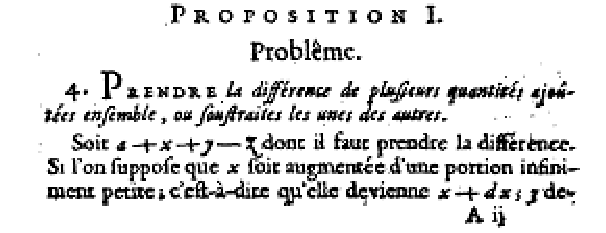
\includegraphics[width=6.5cm]{images/Utilizacion4}
			\par\textbf{PROPOSICI\'{O}N I}
			\par\textbf{Problema}
		\end{center}
		4. TOMAR la diferencia de varias cantidades sumadas,
		o sustra��das ... & %Cambio de columna
		\begin{center}
			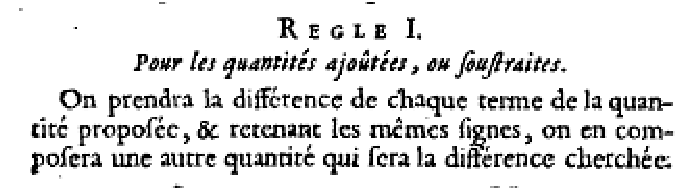
\includegraphics[width=6.5cm]{images/Utilizacion5}
			\par\textbf{REGLA I}
			\par\textbf{\textit{Para las cantidades sumadas o sustra��das}}
		\end{center}
		Tomemos la diferencia de cada t�rmino de la cantidad
		propuesta, y ...\\\hline
	\end{tabular}
	\caption{La tabla muestra el modelo:...}\label{ML:tabla_escalada2}
\end{table}

\end{document}